
%%%%%%%%%%%%%%%%%%%%%%%%%%%%%%%%%%%%%%%%%%%%%%%%%%%%%%%%%%%%%%%%%%%%%%%%%%%%%
%% Descr:       Vorlage für Berichte der DHBW-Karlsruhe, Ein Kapitel
%% Author:      Prof. Dr. Jürgen Vollmer, vollmer@dhbw-karlsruhe.de
%% $Id: kapitel2.tex,v 1.5 2017/10/06 14:02:51 vollmer Exp $
%%  -*- coding: utf-8 -*-
%%%%%%%%%%%%%%%%%%%%%%%%%%%%%%%%%%%%%%%%%%%%%%%%%%%%%%%%%%%%%%%%%%%%%%%%%%%%%%%

\chapter{Systementwurf}
Dieses Kapitel widmet sich dem Systementwurf mit Bezug auf die in Kapitel 1 dargelegte Aufgabenstellung. Dabei wird die Softwarekonzeption 
dargestellt und Gründe für die Wahl der Frameworks genannt. 

\section{Architekturkonzept (Simon Leitl)}
Um Schaltpläne in der Gebäudetechnik, durch die Software zu realisieren, muss ein geeignetes Konzept, sowie ein erster Entwurf erstellt 
werden. Dieser wird als Basis für die künftigen Weiterentwicklungen verwendet. Die Anwendung muss in der Lage sein, auf Benutzerbedienungen 
zu reagieren, Skizzen zeichnen zu können und die Daten passend zu verändern. Wird ein Schaltplan gezeichnet, soll dieser gespeichert und bei 
der nächsten Ausführung wieder geöffnet werden können. Das ermöglicht die mehrmalige Anwendung des Systems für den Nutzer. 
\\Die entstehende Software soll für eine fortführende Entwicklung geeignet sein. Dafür wird ein modularer Aufbau vorgesehen. Dieser soll 
das einfache und schnelle Hinzufügen von Bestandteilen ermöglichen. Des weiteren besteht die Software aus verschiedenen Bestandteilen, die 
oft einzeln behandelt werden. Durch einen modularen Aufbau wird gewährleistet, dass die Module unabhängig voneinander bearbeitet und 
verändert werden können. Ein weiterer Faktor der Systemarchitektur ist das Verhältnis zwischen FrontEnd und BackEnd. Also dem View und der 
Logik. Für eine parallele Entwicklung bietet sich die Entkopplung zwischen der Benutzeroberfläche und der Logik an. Dies hat außerdem den 
Vorteil, dass bei späteren Änderungen der Benutzeroberfläche die Logik nicht angepasst werden muss. Für die entstehende Software wird sowohl 
eine Benutzeroberfläche, sowie eine Datenhaltung und systemweite Verarbeitungsprozesse benötigt. Da als Basissystem \textit{C\#} und das WPF Framework 
benutzt werden, wird für die Architektur das Model-View-ViewModel Pattern ausgewählt. Dieses begünstigt außerdem das Testen der Entwicklung. 
Durch MVVM können UI und BackEnd unabhängig voneinander getestet werden.
\\
Die Software wurde zunächst in zwei große Bausteine geteilt.
\begin{itemize}
    \item Startmenu
    \item Editor
\end{itemize} 
Neben den zwei Bausteinen, verfügt die Anwendung noch über zwei Ordnerstrukturen. Eine für das Speichern von Projekten, die andere für 
die Komponenten, die in das System geladen werden. Die Anwendung im gesamten Überblick ist in Abbildung \ref{pic:softwarearchitektur} 
sichtbar.
\\
\begin{figure}[hbt!]
    \centering
    \includegraphics{4Systementwurf/Bilder/softwarearchitektur}
    \caption{Software-Architektur}
    \label{pic:softwarearchitektur}
\end{figure}
\newpage
\subsection{Startmenü}
Der erste Baustein ist der Einstieg der Anwendung für den Nutzer. Hier wird die Möglichkeit geboten, neue Projekte anzulegen oder bestehende 
Projekte zu öffnen. Dieser soll immer beim Start der Anwendung erscheinen. Dem Nutzer sollen die Optionen über große Schaltflächen auf der 
Benutzeroberfläche zur Verfügung stehen. Das Startmenu zählt daher im ganzen als ein Modul der Software. Der Aufbau des Moduls ist in 
Abbildung \ref{pic:klassendiagramStartmenu} genauer sichtbar. 
\\
\begin{figure}[hbt!]
    \centering
    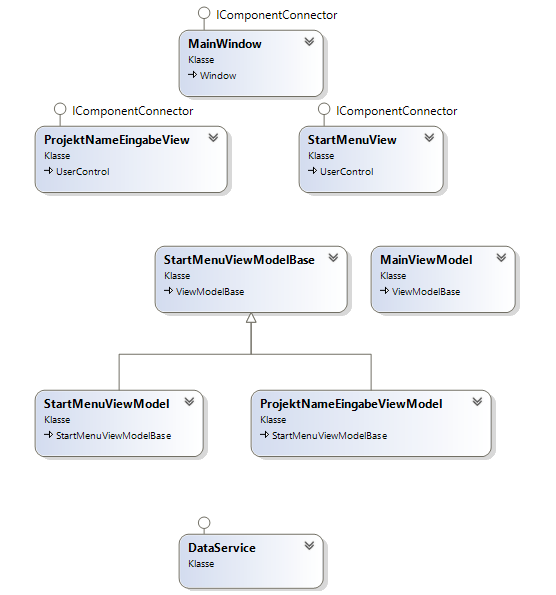
\includegraphics{4Systementwurf/Bilder/klassendiagramStartmenu}
    \caption{Klassendiagramm-Startmenü}
    \label{pic:klassendiagramStartmenu}
\end{figure}
\\ Die Klasse \textit{MainWindow} ist eine XAML Klasse und stellt somit eine Oberfläche dar. Sie bündelt die einzelnen Oberflächen des 
Startmenu. Beim Start der Anwendung öffnet das \textit{MainWindow} die erste Benutzeroberfläche der Software. Die Klasse selbst bindet 
die \textit{StartMenuView.XAML} ein. Diese ist, wie in Abbildung \ref{pic:klassendiagramStartmenu} zu entnehmen, als UserControl angelegt. 
Dies fördert insbesondere den modularen Aufbau der Software. Wird in der zukünftigen Weiterentwicklung etwas an der Startmenu-Komponente 
geändert, so muss nicht das komplette Window verändert werden, sondern ausschließlich der UserControl des Startmenu. Nach MVVM Prinzip 
benötigt das Startmenu-Modul auch eine oder mehrere ViewModel-Klassen, welche die Logik enthalten. Das Startmenu enthält vier 
ViewModel-Klassen:
\begin{itemize}
    \item  \textit{StartMenuViewModelBase}
    \item  \textit{MainViewModel}
    \item \textit{StartMenuViewModel}
    \item \textit{ProjektNameEingabeViewModel}
\end{itemize}  
\textit{StartMenuViewModelBase} und \textit{MainViewModel} erben von der globalen ViewModelBase Klasse, welche bereits in Kapitel 
\ref{chap:MVVM} beschrieben wurden. Sie sind der zentrale Anhaltspunkt für die Logik und beinhalten die Funktionen, welche von der 
Benutzeroberfläche direkt gebindet werden. 
\\Neben den ViewModels, enthält das StartMenu natürlich auch noch ein Model. Dieses ist in Abbildung \ref{pic:klassendiagramStartmenu} 
als \textit{DataService} dargestellt. Die DataService Klasse kümmert sich um die Bereitstellung der Daten. Hier insbesondere um die 
Bereitstellung der vorhandenen Projektdateien, die aufgerufen und geladen werden können.
\\Die zweite Funktion des Startmenus beinhaltet das Erstellen eines neuen Projekts. Dafür dient das ProjektNameEingabeView UserControl. 
Hier hat der Benutzer die Möglichkeit, einen Namen für das neu angelegte Projekt zu definieren. Das Projekt wird dann dementsprechend, mit 
dem vom Benutzer definierten Namen, in einer Ordner-Struktur gespeichert. Mehr zum Ablauf der Speicherung, sowie der Ordner-Struktur ist in 
Kapitel \ref{chap:UseCase-Startmenu} beschrieben. Um das Erzeugen der Datei des neuen Projekts durchzuführen, ist das 
\textit{ProjektNameEingabeViewModel} zuständig. 
\subsection{Editor}
\label{chap:Editor}
Der Editor enthält die eigentlichen Kernfunktionen der Anwendung. Hier sollen die Schaltpläne entstehen. Er erscheint nach dem im Startmenu 
ein neues Projekt angelegt, oder ein bestehendes Projekt ausgewählt wurde. Der Editor stellt eine Zeichenfläche bereit, in der es ermöglicht 
wird Schaltpläne zu skizzieren. Dabei werden durch verschiedene Werkzeugleisten, einzelne Komponenten zur Auswahl gestellt. Diese sind 
Notwendig um einen Schaltplan zu erstellen. Das Editor Fenster selbst, besteht aus einzelnen UserControls, um künftige Änderungen an der 
Oberfläche zu gewährleisten, ohne das diese Änderungen an den restlichen Elementen auslösen. Auch im Editor wird wieder nach dem Schema des 
MVVM Patterns vorgegangen. Dabei wird für jeden einzelne Element der Oberfläche, welche in UserControls angelegt werden, eigene ViewModels 
sowie Models erstellt. Beispielsweise enthält der Editor ein UserControl, der Werkzeuge zum Zeichnen der Leitungen bereitstellt. Nach MVVM 
wurden hier die folgenden Klassen erzeugt:
\begin{itemize}
    \item \textit{LeitungenToolsView}  
    \item \textit{LeitungenToolsViewModel} 
    \item \textit{LeitungenToolsModel}
\end{itemize}
Der Editor umfasst 
Alle User Controls des Editors werden in Kapitel \ref{chap:Softwarekonzept} genauer beschrieben.
\subsection{Programmier Richtlinien}
Um eine Übersichtlichkeit innerhalb des Projekts zu schaffen, damit auch künftig Entwickler, Änderungen an der Anwendung vornehmen können, wurden zu Beginn einige Richtlinien für die Programmierung und den Programmierstil festgelegt. 
\begin{itemize}
    \item Klassen, Variablen und Funktionen sollen aussagekräftige Namen erhalten. Wenn Möglich sollen die Namen den Inhalt bzw die Funktion der Klasse, Variable und Funktion beschreiben. 
    \item Klassen, Variablen und Funktionen die unterschiedliche Inhalte und Funktionen beinhalten, dürfen keinen ähnlichen Namen enthalten. Die Namen sollen für die Entwickler eindeutig unterscheidbar sein. 
    \item Aufgrund der Benutzung des MVVM Patterns, sind für Bestandteile der Anwendung meist drei Klassen enthalten. \textit{View, ViewModel, Model}. Die zugehörigen Klassen erhalten den gleichen Namen und unterscheiden sich lediglich in der Endung. Z.b. \textit{StartMenuView, StartMenuViewModel, StartMenuModel}.
\end{itemize} 
Diese Richtlinien dienen als Leitfaden für Entwickler. Sie sind an das Konzept Clean-Code angelehnt. 
\subsection{Mockups (Mikka Jenne)}
% https://www.degruyter.com/downloadpdf/books/9783110443882/9783110443882-005/9783110443882-005.pdf[3]
% https://www.gruenderszene.de/lexikon/begriffe/user-experience?interstitial [2]
% Foliensatz Advanced Software Engineering Maurice Müller Usability & UX
Bei der Entwicklung des allgemeinen Architekturkonzepts wurden parallel dazu auch erste grafische Entwürfe für die Darstellung der Benutzeroberflächen erstellt.
Dabei wurden User-Experience und Usability Faktoren berücksichtigt. \cite{gruenderszene.2020m}
\\
Die \ac{UX} umfasst alle Berührpunkte eines Nutzers mit einem Produkt, 
Dienstleistung oder Service. Sie spiegelt Erfahrungen sowie auch Empfindungen und Gefühle einer Person während der Benutzung eines Produktes wieder. \cite{foliensatz.2020m}
\\Usability (dt. Gebrauchstauglichkeit), ist ein Teil der User-Experience der speziell auf die exakte Gebrauchstauglichkeit der Anwendung, Dienstleistung
o.ä. abzielt. Dabei zu beachtende Faktoren sind unter anderem der Aufgabe, der Problemlösung angemessen und z.B. verständliche Anweisungen. 
\linebreak
Die für uns wichtigsten Faktoren der User-Experience und Usability wurden aus einer Menge bestehender Merkmale selektiert und während des Designs berücksichtigt. Diese Aspekte werden in
folgender Auflistung erläutert. \cite{degruyter.2020m}
\\
\linebreak
\begin{itemize}
    % \item Durchschaubarkeit
    % \begin{itemize}
        % \item Erlernbarkeit, Lernförderlichkeit
        % \item Ist es einfach, die Bedienung des Produkts zu verstehen und zu erlernen? Quelle: ISO 9241 (Teil 110 – dort als Lernförderlichkeit bezeichnet).
    % \end{itemize}
    \item Effizienz
    \begin{itemize}
        \item Der Nutzer kann seine Ziele mit minimalem zeitlichem und physischem Aufwand
        erreichen. Das Produkt reagiert schnell auf Nutzereingaben. Das Design der
        Nutzerschnittstelle macht keine unnötigen Arbeitsschritte erforderlich. Quelle: ISO 9241
        (Teil 11) bzw. (Teil 110 – Aufgabenangemessenheit).
    \end{itemize}
    % \item Immersion
    % \begin{itemize}
        % \item Wenn der Nutzer sich mit dem Produkt beschäftigt, vergisst dieser die Zeit. Der
        % Nutzer kann völlig in der Beschäftigung mit dem Produkt versinken. Dieses
        % Qualitätskriterium ist insbesondere bei Spielen und anderen zur Unterhaltung dienenden
        % Produkten relevant.
    % \end{itemize}
    \item Intuitive Bedienung
    \begin{itemize}
        \item Kann der Nutzer die Benutzerschnittstelle mit seinen vorhandenen
        Fähigkeiten unmittelbar und ohne jegliche Einarbeitung oder Anleitung durch andere
        bedienen? Quelle: Mohs et al. (2006).
    \end{itemize}
   % \item Leichtigkeit 
    %\begin{itemize}
    %    \item Es ist für den Nutzer einfach seine Aufgaben mit dem Produkt zu erledigen. 
    %    Die Interaktion mit dem Produkt ist weder körperlich noch mental anstrengend. Quelle: Hart und Staveland (1988) NASA-TLX (Task Load Index).
    %\end{itemize}
    %\item Nützlichkeit
    %\begin{itemize}
    %    \item Die Benutzung des Produkts bringt Vorteile. 
    %    \item Z.B. Produktivität und Effizienz bei Prozessen.
    %\end{itemize}
    %\item Schönheit
    %\begin{itemize}
    %    \item Ästhetik
    %    \item Das Produkt ist schön und ansprechend gestaltet. Das Produkt macht auf den Nutzer einen ästhetischen Eindruck.
    %\end{itemize}
    %\item Steuerbarkeit  
    %\begin{itemize}
    %    \item Kontrollierbarkeit, Fehlertoleranz, Robustheit
    %    \item Das Produkt reagiert immer vorhersehbar und konsistent auf Nutzerinteraktionen. Der Nutzer hat stets die volle Kontrolle über das Produkt. Quelle: ISO 9241 (Teil 110).
    %\end{itemize}
    %\item Übersichtlichkeit  
    %\begin{itemize}
    %    \item Visuelle Komplexität
    %    \item Die Benutzerschnittstelle wirkt aufgeräumt und übersichtlich und hat eine geringe visuelle Komplexität. Der Nutzer findet sich schnell darin 
    %    zurecht. Quelle: Müller und Schrepp (2013).
    %\end{itemize}
    %\item Vertrauen 
    %\begin{itemize}
    %    \item Die Daten und Informationen, die der Nutzer bei der Interaktion mit dem
    %    Produkt eingibt, sind in sicheren Händen. Dies spielt natürlich vor allem bei Produkten eine
    %    Rolle, bei denen der Nutzer kritische Daten preisgibt, z.B. beim Einkaufen in Web-Shops
    %    oder Online-Banking. Quelle: Corritore et al. (2001).
    %\end{itemize}
    \item Vollständigkeit 
    \begin{itemize}
        \item Das Produkt bietet dem Nutzer alles, was er oder sie erwartet. Es fühlt sich
        vollständig an, auch wenn es nicht tatsächlich alles im konkreten Nutzungskontext
        Notwendige bieten sollte. Der Faktor Vollständigkeit bezieht sich somit mehr auf die
        wahrgenommene Vollständigkeit und weniger auf die Summe der aufgabenangemessenen
        Nutzungskontexte. 
    \end{itemize}
\end{itemize}
Anhand der aufgelisteten Faktoren und der 
Umschreibung des zu lösenden Problems der 
Schaltplanzeichnung sind die aufgeführten Abbildung
4.3 und Abbildung 4.4 entstanden, die es galt in der Implementierung möglichst abbildungsgetreu wiederzugeben.
\pagebreak
\begin{figure}[htb]
    \section*{Startmenü Mockup}
    \centering
    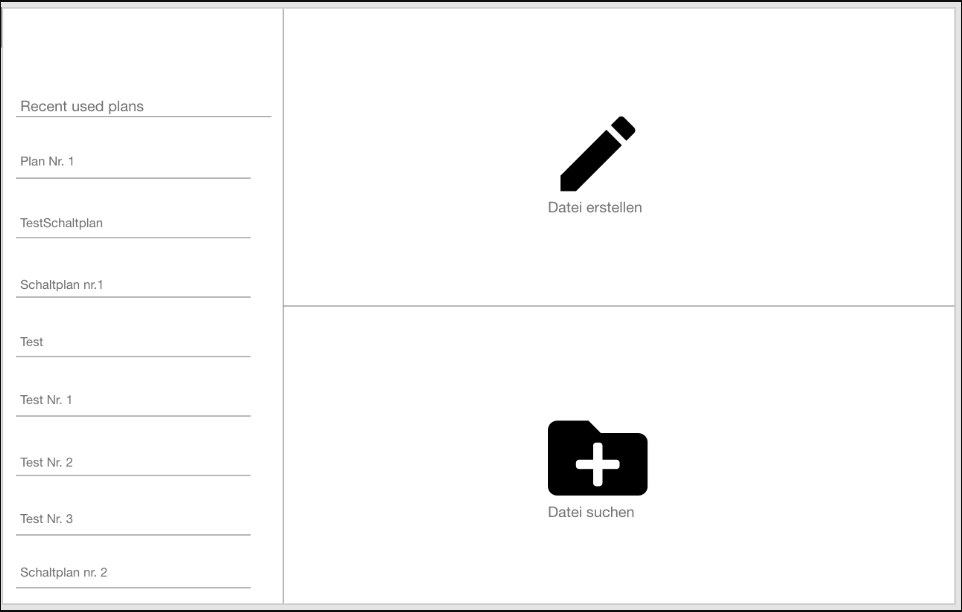
\includegraphics[width=15cm,height=10cm]{4Systementwurf/Bilder/StartMenuViewMockUp}
    \caption{Startmenü Mockup}
    \label{StartMenuViewMockUp}
\end{figure}
\\Die Benutzeroberfläche des Startmenüs ist einfach und selbsterklärend aufgebaut, sodass ohne große Worte der Umgang 
und der weitere Verlauf des Programms selbsterklärend ist. Die Oberfläche ist sichtlich in drei Rubriken eingeteilt, womit 
die wichtigsten Starteigenschaften 
repräsentiert werden.
\\
\linebreak
Über die in Abbildung 4.3 dargestellte Auflistung, getitelt mit \textit{Recent used plans}, werden alle erstellten Dokumente als Schnellzugriff zur
Verfügung gestellt. Jede einzelne Datei kann über diesen Menüpunkt aufgerufen und im Editor geöffnet werden. Zudem bietet diese Auflistung 
eine schnelle Übersicht über alle erstellten Dokumente. 
\\
\linebreak
Das rechte obere Drittel des Bildes stellt den Service zum Erstellen einer neuen Datei zur Verfügung. Durch klicken des Bildes, bzw. 
der Fläche wird das eigentliche Programm angestoßen, welches in dem Kapitel 5 Implementierung ausführlich erläutert und dargelegt wird.
\\
\linebreak
Das rechte untere Drittel weißt darauf hin einen Ordner öffnen zu können, damit vorhandene Dateien, 
z.B. aus anderen Ordnern, geöffnet und geladen werden können. Die genaue Vorgehensweise, bzw. die implementierten Funktionen
werden ebenso in Kapitel 5 genauestens dargestellt. 
\pagebreak
\\Ein simples Layout zum Start der Applikation, während die Editoransicht, der eigentliche Kern der Anwendung, deutlich 
mehr Funktionen und Möglichkeiten bietet.
Um die Abbildung 4.4 besser deuten zu können, wird nach Aufführung des Bildes eine Erklärung und eine kurze Begründung, wieso 
das Layout so gewählt wurde, stattfinden.
\\
\begin{figure}[htb]
   \section*{Editor Mockup}
   \centering
  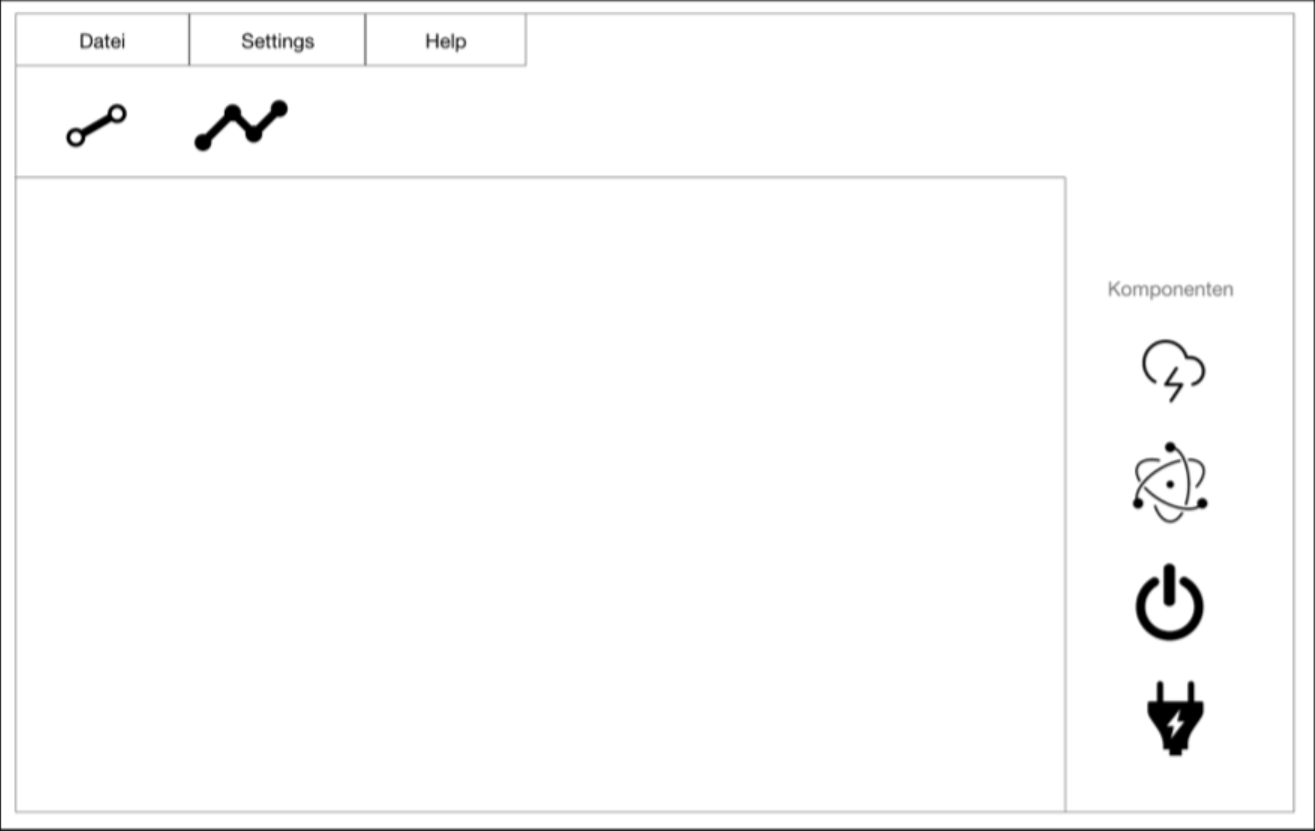
\includegraphics[width=15cm,height=10cm,keepaspectratio]{4Systementwurf/Bilder/EditorViewMockUp.png}
 \caption{Editor Mockup}
\end{figure} % https://www.wpftutorial.net/Canvas.html 
\\Wie in der Abbildung zu sehen ist, wird zentral eine weiße Fläche dargestellt. Diese Fläche repräsentiert ein Canvas, welches für die
Zeichnung der Schaltpläne geeignet ist. 
\\Das Canvas in WPF ist das grundlegendste Layout-Fenster für das Zeichnen von Objekten. Durch explizite Koordinaten können Elemente und 
Objekte in diesem Fenster positioniert werden. Die Koordinaten können relativ zu jeder Seite des Bedienfeldes im Canvas-Bereich angegeben 
werden.
\\
\linebreak
Die Oberfläche ist aufgeteilt in drei Segmente. Dies sind die Zeichenfläche als primäre Funktion, die zur Verfügung stehenden 
Komponenten zum Zeichnen angeordnet um das Canvas herum und die allgemeinen Einstellungen und Optionen als Reiterflächen im linken 
oberen Bereich. 
\\
\linebreak
Das entwickelte Design ist stark an andere bekannte Softwaredesigns, wie z.B. Microsoft Word, angelehnt, da dies ein gewohntes
Format ist und der Nutzer ungefähr, weiß wie das Programm zu benutzen ist, um schnell auf einen Fortschritt oder ein Ergebnis zu kommen. 
Trotz der Anlehnung an MS Word weicht es doch vom Design ab und kann damit nicht direkt und eindeutig verglichen werden. 
Vergleichbar sind z.B. die symbolisierten Flächen zum Auswählen verschiedenster Tools und Komponenten, die Einstellungsrubriken und 
die eigentliche Designfläche.
\section{Softwarekonzept (Simon Leitl)}
\label{chap:Softwarekonzept}
Im folgenden werden die einzelnen Bestandteile des in Kapitel \ref{chap:Editor} beschriebenes Editor, genauer erläutert. 
\begin{figure}[hbt!]
    \centering
    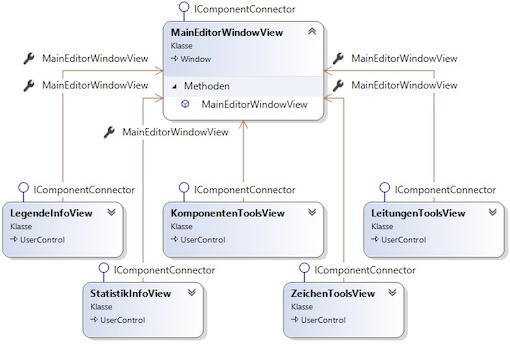
\includegraphics{4Systementwurf/Bilder/EditorView}
    \caption{Editor-viewKlassendiagramm}
    \label{pic:viewKlassendiagramm}
\end{figure}
\linebreak
Alle Bestandteile werden als UserControls in das MainEditorWindow eingebunden. Somit repräsentiert ein Fenster die verschiedenen Funktionen. Für die Implementierung sind diese jedoch abgekoppelte Bestandteile. Jedes UserControl kann einzeln und selbständig programmiert und gestaltet werden. Daher werden diese im Klassendiagramm (Abb. \ref{pic:viewKlassendiagramm}) als einzelne Klassen aufgeführt, mit Zuordnung zum MainEditorWindow. 
\subsection{Zeichenfläche}
Die Zeichenfläche ist der größte Bestandteil des Editors. Hier hat der Nutzer die Möglichkeit einen Schaltplan zu zeichnen. Dabei wählt er zunächst in den Werkzeugleisten ein Werkzeug aus. Wählt er beispielsweise ein Werkzeug zum zeichnen des Grundrisses aus den ZeichenTools aus, hat er die Möglichkeit innerhalb der Zeichenfläche einen Grundriss zu zeichnen. 
\subsection{KomponentenTools}
Die KomponentenTools sind eine Werkzeugleiste, welche dem Benutzer die für einen Schaltplan benötigten elektrischen Komponenten zur Verfügung stellt. Solche sind zum Beispiel eine Steckdose oder eine Leuchte. Die Komponenten verfügen über einen Namen sowie ein Symbol, um sie eindeutig zu identifizieren. Das Symbol einer Komponente wird später im Schaltplan angezeigt, sofern es benutzt wird.
\subsection{LeitungenTools}
Die LeitungenTools sind eine weitere Werkzeugleiste, welche dem Benutzer die für einen Schaltplan benötigten Leitungen zur Verfügung stellen. Hierbei gibts es folgende Leitungen zur Auswahl. 
\begin{itemize}
    \item 3 x 1,5mm 
    \item 3 x 2,5mm
    \item 5 x 1,5mm
    \item 5 x 2,5mm
\end{itemize}
Alle Leitungen werden durch unterschiedliche Farben und Formen gekennzeichnet, damit sie im Schaltplan eindeutig und schnell erkannt werden. 
\subsection{ZeichenTools}
Die ZeichenTools sind eine weitere Werkzeugleiste im Editor, welche zum Zeichnen der Gebäudeumrisse dienen. Sie bieten verschiedene Darstellungen und Formen um Gebäude zeichnerisch korrekt darzustellen.
\subsection{LegendeInfo}
Die LegendeInfo ist ein Bestandteil des Editors, welcher eine Legende zum Schaltplan darstellt. Die Legende dient dazu den Schaltplan zu lesen und zu verstehen. Sie stellt die Bedeutung von Symbolen dar. So kann der Schaltplan auch schnell von dritten, die ihn nicht erstellt haben, überblickt werden.
\subsection{StatistikInfo}
Die StatistikInfo ist ein Bestandteil des Editors, welcher eine Übersicht über die verwendeten Werkzeuge und Komponenten darstellt. Die Statistik soll dem Benutzer einen Überlick verschaffen, wie viele Werkzeuge bzw. Komponenten er in seiner Zeichnungen benutzt hat. Hat er beispielsweise vier Steckdosen in der Zeichnung angebracht, so zeigt ihm die Statistik an, dass vier Steckdosen verwendet wurden. Dies erspart dem Benutzer das abzählen innerhalb der Skizze.
%\begin{wrapfigure}{l}{0.4\textwidth}
%\fbox{
\includegraphics[width=0.25\textwidth,angle=270]{lion}}
%\end{wrapfigure}


%%%%%%%%%%%%%%%%%%%%%%%%%%%%%%%%%%%%%%%%%%%%%%%%%%%%%%%%%%%%%%%%%%%%%%%%%%%%%%%
